% Please do not create a heading level below \subsection. For 3rd level headings, use \paragraph{}.
%
% % % % % % % % % % % % % % % % % % % % % % %
%
% -- FIGURES AND TABLES
%
% Please include tables/figure captions directly after the paragraph where they are first cited in the text.
%
% DO NOT INCLUDE GRAPHICS IN YOUR MANUSCRIPT
% - Figures should be uploaded separately from your manuscript file.
% - Figures generated using LaTeX should be extracted and removed from the PDF before submission.
% - Figures containing multiple panels/subfigures must be combined into one image file before submission.
% See http://www.plosone.org/static/figureGuidelines for PLOS figure guidelines.
%
% Tables should be cell-based and may not contain:
% - tabs/spacing/line breaks within cells to alter layout or alignment
% - vertically-merged cells (no tabular environments within tabular environments, do not use \multirow)
% - colors, shading, or graphic objects
% See http://www.plosone.org/static/figureGuidelines#tables for table guidelines.
%
% For tables that exceed the width of the text column, use the adjustwidth environment as illustrated in the example table in text below.
%
% % % % % % % % % % % % % % % % % % % % % % % %
%
% -- EQUATIONS, MATH SYMBOLS, SUBSCRIPTS, AND SUPERSCRIPTS
%
% IMPORTANT
% Below are a few tips to help format your equations and other special characters according to our specifications. For more tips to help reduce the possibility of formatting errors during conversion, please see our LaTeX guidelines at http://www.plosone.org/static/latexGuidelines
%
% Please be sure to include all portions of an equation in the math environment.
%
% Do not include text that is not math in the math environment. For example, CO2 will be CO\textsubscript{2}.
%
% Please add line breaks to long display equations when possible in order to fit size of the column.
%
% For inline equations, please do not include punctuation (commas, etc) within the math environment unless this is part of the equation.
%
% % % % % % % % % % % % % % % % % % % % % % % %
%
% Please contact latex@plos.org with any questions.
%
% % % % % % % % % % % % % % % % % % % % % % % %

\documentclass[10pt,letterpaper]{article}
\usepackage[top=0.85in,left=2.75in,footskip=0.75in]{geometry}

% Use adjustwidth environment to exceed column width (see example table in text)
\usepackage{changepage}

% Use Unicode characters when possible
\usepackage[utf8]{inputenc}

% textcomp package and marvosym package for additional characters
\usepackage{textcomp,marvosym}

% fixltx2e package for \textsubscript
\usepackage{fixltx2e}

% amsmath and amssymb packages, useful for mathematical formulas and symbols
\usepackage{amsmath,amssymb}

% cite package, to clean up citations in the main text. Do not remove.
% \usepackage{cite}

% Use nameref to cite supporting information files (see Supporting Information section for more info)
\usepackage{nameref,hyperref}

% line numbers
% \usepackage[right]{lineno}

% ligatures disabled
\usepackage{microtype}
\DisableLigatures[f]{encoding = *, family = * }

% rotating package for sideways tables
\usepackage{rotating}

% writing SI units
\usepackage{siunitx}

% include graphics
\usepackage{graphicx}
\graphicspath{ {images/} }

% place float at precise locations (for figures)
\usepackage{float}

% handle references
\usepackage[backend=biber,style=alphabetic,style=nature]{biblatex}
\addbibresource{reference.bib}

% Remove comment for double spacing
%\usepackage{setspace}
%\doublespacing

% Text layout
\raggedright
\setlength{\parindent}{0.5cm}
\textwidth 5.25in
\textheight 8.75in

% Bold the 'Figure #' in the caption and separate it from the title/caption with a period
% Captions will be left justified
\usepackage[aboveskip=1pt,labelfont=bf,labelsep=period,justification=raggedright,singlelinecheck=off]{caption}

% % Use the PLoS provided BiBTeX style
% \bibliographystyle{plos2009}
%
% % Remove brackets from numbering in List of References
% \makeatletter
% \renewcommand{\@biblabel}[1]{\quad#1.}
% \makeatother

% Leave date blank
\date{}

% Header and Footer with logo
\usepackage{lastpage,fancyhdr,graphicx}
\pagestyle{myheadings}   % footer is empty by default
\pagestyle{fancy}
\fancyhf{}
\lhead{
\includegraphics[natwidth=1.3in,natheight=0.4in]{PLOSlogo.png}}    % left header
\rfoot{\thepage/\pageref{LastPage}}   % right footer   \pageref{LastPage} access total number of pages
\renewcommand{\footrule}{\hrule height 2pt \vspace{2mm}}
\fancyheadoffset[L]{2.25in}
\fancyfootoffset[L]{2.25in}
\lfoot{\sf PLOS}

%% Include all macros below

% \newcommand{\lorem}{{\bf LOREM}}
% \newcommand{\ipsum}{{\bf IPSUM}}

%% END MACROS SECTION


\begin{document}
\vspace*{0.35in}

% Title must be 150 characters or less
\begin{flushleft}
{\Huge
\textbf\newline{Amplification of PITPNC1 affects breast cancer progression
}
}
\newline
% Insert Author names, affiliations and corresponding author email.
\\\textbf{\sffamily
Peiqi Wang\textsuperscript{1},
Ranju Nair\textsuperscript{3,4},
Nisha Kanwar\textsuperscript{2,3,4},
Grace Cheung\textsuperscript{4},
Susan J. Done\textsuperscript{2,3,4,*}
}
\newline
\\\footnotesize{\sffamily
{\bfseries 1} Department of Molecular Genetics and Microbiology, University of Toronto, Toronto, ON, Canada. {\bfseries 2} Department of Laboratory Medicine and Pathology, University of Toronto, Toronto, ON, Canada. {\bfseries 3} The Campbell Family Institute for Breast Cancer Research, Toronto, ON, Canada. {\bfseries 4} University Health Network, Toronto, ON, Canada {\bfseries *} Susan.Done@uhn.ca}
\end{flushleft}


{\bfseries\sffamily
\noindent In our previous array comparative genomic hybridization studies, gain in a region of chromosome 17, 17q23.3-24.3, was frequently observed in invasive duct carcinoma (IDC) patients with lymph node metastasis. Particularly, phosphatidylinositol transfer protein, cytoplasmic 1 (PITPNC1), found in 17q24.2, was associated with higher histological grade, larger tumor size, positive HER2 staining, and poorer prognosis from the analysis of a NKI dataset. PITPNC1 is involved in signal transduction and intracellular lipid transport, and may be an essential part of the epidermal growth factor signaling pathway. We aim to assess the role of PITPNC1 in the development of aggressive breast cancer by evaluating its effects on breast cancer progression. Using real-time PCR, we have validated PITPNC1 overexpression in a set of 26 ductal carcinoma in situ (DCIS) and 38 invasive ductal carcinoma (IDC) samples. Amplification of PITPNC1 was seen as early as DCIS and persisted to IDC. PITPNC1 overexpressing MDA-MB-231 exhibited higher proliferation than transfection controls. Further characterization of PITPNC1 protein function, especially during the course of tumorigenesis and cancer progression, may yield promising insights to cancer biology and early diagnostics.
}

\section*{Introduction}
Breast cancer is one of the leading cause of cancer related death amongst women. In 2016, 61,000 new cases of non-invasive breast cancer and 246,660 new cases of invasive breast cancer are expected to be diagnosed in U.S. alone. \cite{1_siegel_miller_jemal_2016} Identification of molecular alterations associated with breast cancer progression is crucial for tailoring individualized treatments and enhancing prognostic confidence.

Current model of breast cancer progression consists of a multistep process: from pre-malignant ductal hyperplasia (DH) to non-invasive ductal carcinoma in situ (DCIS), which develops into invasive ductal carcinoma (IDC) of similar tumor grade. \cite{2_bombonati_sgroi_2010} Despite advances in characterizing molecular alterations in IDC, few studies focused on disease initiation and progression. Several gene expression studies have shown striking similarity in DCIS and IDC transcriptome profile, indicating that molecular heterogeneity of breast carcinomas is already established in DCIS \cite{3_ma_salunga_tuggle_gaudet_enright_mcquary_payette_pistone_stecker_zhang,10_porter_lahti-domenici_keshaviah_bae_argani_marks_richardson_cooper_strausberg_riggins}. Although key genetic alterations responsible for DCIS to IDC transition are not easily distinguishable, dramatic expression changes were seen in the normal epithelial to DCIS transition. \cite{10_porter_lahti-domenici_keshaviah_bae_argani_marks_richardson_cooper_strausberg_riggins} To account for variable clinical outcome of DCIS patients, expression profiling of DCIS suggested that tumor grade, rather than tumor stage, is linked to distinct expression patterns. \cite{3_ma_salunga_tuggle_gaudet_enright_mcquary_payette_pistone_stecker_zhang} Some reported a panel of differentially expressed genes to aid in stratifying DCIS and progression to IDC of corresponding tumor grade, but no single markers were found to predict DCIS outcome. \cite{9_hannemann_velds_halfwerk_kreike_peterse_van} Combining these points, it may be tempting to identify biologically relevant alterations that are predictive of invasion early in breast cancer progression.

Breast cancer has been known to suffer from constant genomic arrangement during its development. Marked increase in genomic instability - specifically amplifications, deletions, and complex translocations - were observed in the DH to IDC transition early in breast cancer development. \cite{15_depinho_polyak_2002} Although it is well established that breast tumors most frequently experience gains on chromosome 8q, 11q, 17q, and 20q, the copy number alterations of DCIS is broadly similar to that of IDC. \cite{17_chin_devries_fridlyand_spellman_roydasgupta_kuo_lapuk_neve_qian_ryder,18_kallioniemi_kallioniemi_piper_tanner_stokke_chen_smith_pinkel_gray_waldman_1994,21_gorringe_hunter_pang_opeskin_hill_rowley_choong_thompson_dobrovic_fox} Differing gains and losses were identified in the DCIS to IDC transition, prompting an urgent need to verify and characterize these copy number alternations. \cite{22_johnson_gorringe_thompson_opeskin_boyle_wang_hill_mann_campbell_2012,23_hernandez_wilkerson_lambros_campion_flora_rodrigues_gauthier_cabral_pawar_mackay_a_hern} In a previous array comparative genomic hybridization (aCGH) study, gain of a region on chromosome 17, 17q23.3-24.3, was frequently observed in DCIS with IDC compared to pure DCIS and was found to be associated with lymph node metastasis. \cite{11_iakovlev_arneson_wong_wang_leung_iakovleva_warren_pintilie_done_2008} To identify causative genes in within the 17q23.3-24.3 amplicon, we identified phosphatidylinositol transfer protein, cytoplasmic 1 (PITPNC1), found on 17q24.2, to be associated with higher histological grade, larger tumor size, positive HER2 staining, and poor prognosis by analyzing a NKI dataset (n = 295).

As a part of the phosphatidylinositol transfer protein family, PITPNC1 has been shown to be an essential component of phosphatidylinositol-4,5-bisphosphate (PIP2) synthesis machinery. \cite{12_liscovitch_cantley_1995} PITPNC1 also mediates the monomeric transport of lipids by shielding phosphatidylinositol in a hydrophobic cavity, transferring them between membrane bilayers. Although its exact function has not been verified, PITPNC1 may be involved in the epidermal growth factor signaling pathway, by providing the substrate for phosphatidyl-4,5-bisphosphate 3-kinase (PI3K) catalysis and facilitating the downstream activation of protein kinase B (Akt). PITPNC1 was also implicated as a target of miR-126, a tumor suppressing non-coding microRNA. Expression of PITPNC1 is strongly correlated with endothelial recruitment in vitro and is associated with late pathological stage. \cite{13_png_halberg_yoshida_tavazoie_2011}

Here we hypothesized that amplification of PITPNC1 may be responsible for increased invasive potential of DCIS. We aim to validate PITPNC1 expression profile in a cohort of breast cancer patients cross successive tumor stages. We also aim to assess the role of PITPNC1 in the development of aggressive breast cancer by evaluating its functional significance in vitro, specifically its influence on cell proliferation, migration and invasion.

\section*{Methods}
\subsection*{Clinical sample preparations}
A total of 89 patient samples – 25 derived from normal breast tissue, 26 DCIS, and 38 IDC from primary sites - were included for this study.  With approval from University Health Network Research Ethics Ethics Board, formalin-fixed paraffin-embedded (FFPE) breast cancer tissue blocks were obtained from Princess Margaret Hospital. Cancerous tissues on the slides were marked and microdissected using a stereomicroscope and 18 gauge needles. DNA were extracted using a Qiagen DNA Mini Kit and genome amplified using ligation-mediated PCR (SCOMP) following manufacturer’s protocol.

\subsection*{Quantitative real-time PCR }
Patient samples were diluted to 1 \si{\nano\gram\per\micro\litre} and subjected to quantitative real-time PCR. Each patient sample was prepared as a technical triplicate and amplified using primers targeting PITPNC1 as well as, separately, the housekeeping gene B2M. Amplification of DNA was quantitated with SYBR Green probe using 7900HT Real-Time PCR System (Applied Biosystems) in a 384-well plate. qPCR was also performed on a set of normal breast controls – 7 SCOMP amplified, 9 whole genome amplified, and 8 unamplified samples – to validate the efficacy of SCOMP amplification method as well as to generate a baseline for statistical comparison. Sequences of PCR primer pairs are as follows:

\vspace*{1\baselineskip}
\hspace*{10mm} $PITPNC1$
\\\hspace*{20mm}$\text{forward } TGCCGAAATTCTCCATTCATATAG$
\\\hspace*{20mm}$\text{reverse } TACTCAGGTGTCATTGCTTCCT$
\\\hspace*{10mm} $B2M$
\\\hspace*{20mm}$\text{forward } GCTCCCGATCTTCTCAGTTTAG$
\\\hspace*{20mm}$\text{reverse } CGCGCGTACCTATGCTATATT$

\subsection*{Statistical Analysis}
Copy number alterations of PITPNC1 were analyzed using Livak method. Raw data was imported to R and normalized to respective B2M threshold cycles as well as a to an invariant normal breast sample calibrator present in every plate. Copy number alterations were expressed as relative fold difference against controls used. Pairwise determination of statistical significance was calculated using Welch two-sample t-test. All plots / graphs were generated using R/ggplot2.

\subsection*{Cell Line and transfection}
Cell lines were maintained in 10$\%$ fetal bovine serum with DMEM (Dulbecco’s Modified Eagle Medium). Viral vectors overexpressing PITPNC1 as well as empty viral vector were transfected into HEK293. Viral particles were harvested and subsequently transduced into the invasive MDA-MB-231 cell line.

\subsection*{Proliferation and Invasion/Migration Assays}
250 cells from PITPNC1 overexpressing MDA-MB-231 cell line as well as transfection controls were plated and incubated for three days. Proliferation capabilities associated with PITPNC1 overexpression were evaluated using a hemocytometer on cells stained with Trypan blue. Migration and invasion potentials were tested using a Trans-well migration assay. A total of 1000 cells were added to the top chamber with 8.0 micrometer pore membrane. After 24 hours of incubation, the cells migrated to the other side of the membrane were stained using Diff-Quick and counted.

\newpage
\section*{Results}

\subsection*{PITPNC1 is amplified in DCIS and IDC FFPE samples}
To verify that amplification of PITPNC1 corresponds to microarray data, we used qPCR to quantitate PITPNC1 fold differences in SCOMP amplified FFPE samples. To ensure the validity of qPCR on amplified FFPE DNA samples, we first tested the fidelity of SCOMP amplification method by comparing PITPNC1 copy number alterations in 7 SCOMP amplified, 9 WGA amplified, and 8 unamplified normal breast tissues (Figure ~\ref{fig1}). In general, genome amplification methods reduce the number of detectable PITPNC1 to within one threshold cycle when compared to unamplified DNA. Measurements from SCOMP amplified samples were close to that of WGA amplified sample, reinforcing the reproducibility of qPCR analysis on SCOMP amplified FFPE DNA. Although we tried to select matched DCIS and IDC from the same patient section, no statistically significant conclusion was derived from these matched cases because of insufficient sample size. As a result, tumor stage was the only differentiating factor in evaluating copy number alterations of these patient samples. We compared PITPNC1 copy number changes in 26 DCIS and 38 IDC samples against 25 normal breast tissue controls. PITPNC1 was shown to be amplified in DCIS (p=0.0002) and IDC (p=0.05), whose respective 95\% confidence intervals for PITPNC1 fold difference are [3.92, 7.13] and [2.17, 4.94] respectively (Figure ~\ref{fig2}). The large standard error observed may be caused by the inherent heterogeneous nature of malignant breast cancer genome.

\vspace*{2\baselineskip}
\begin{figure}[H]
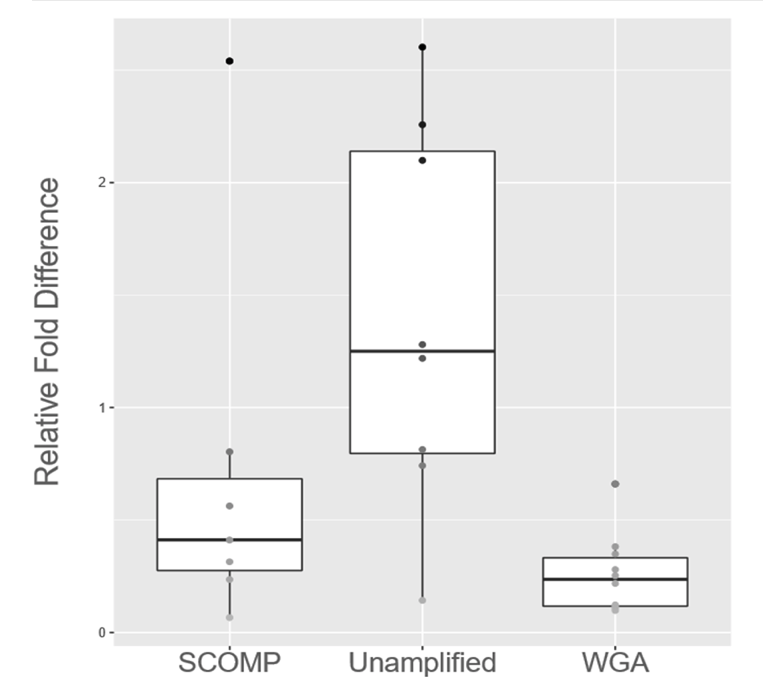
\includegraphics[width = 9cm]{fig1}
\centering
\vspace*{1\baselineskip}
\caption{{\bf SCOMP amplification moderately alters qPCR results}
Comparison of PITPNC1 amplification on normal patient samples prepared with varying amplification methods.  Data were derived from a subset of 7 SCOMP, 9 WGA, and 8 unamplified samples
}
\label{fig1}
\end{figure}
\vspace*{1\baselineskip}
\begin{figure}[H]
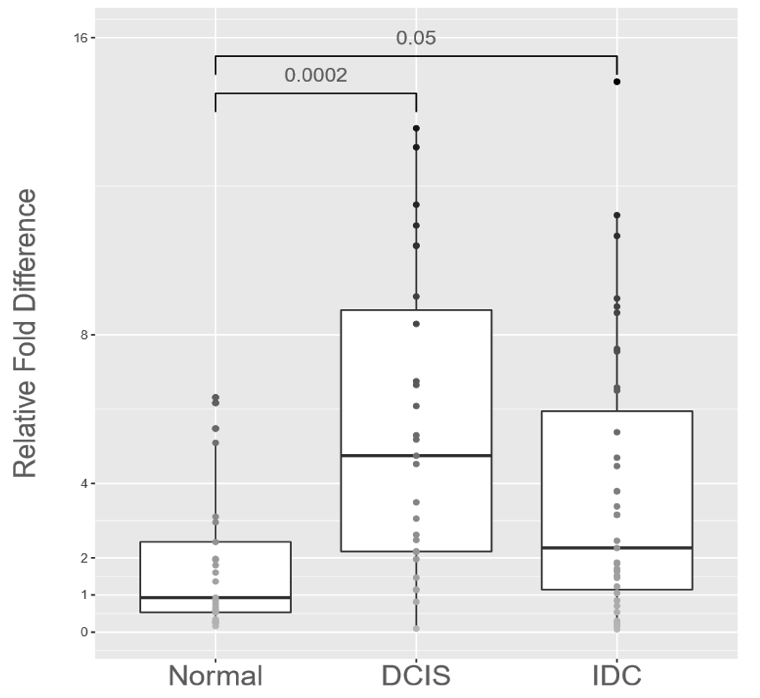
\includegraphics[width = 9cm]{fig2}
\centering
\vspace*{1\baselineskip}
\caption{{\bf PITPNC1 is overexpressed in DCIS and IDC compared to control }
Comparative qPCR analysis on relative expression of PITPNC1 between normal breast tissue controls, DCIS, and IDC samples. Boxplot represents median expression fold differences of the gene. Each dot represents a unique sample, averaged from a triplicate. P-values obtained from Welch two-sample t-test are labeled
}
\label{fig2}
\end{figure}
\vspace*{2\baselineskip}

\subsection*{Overexpression of PITPNC1 promotes cell proliferation \textit{in vitro}}
Since PITPNC1 is amplified in DCIS and IDC, we asked if PITPNC1 has a functional effect on breast cancer cell line. To verify this hypothesis, we tested whether overexpression of PITPNC1 in basal MDA-MB-231 cells promote cell proliferation. We generated cell line stably overexpressing PITPNC1 via viral transduction (Figure ~\ref{fig3}). Overexpression of PITPNC1 strongly stimulates cell division (Figure ~\ref{fig4}). As migration and invasion are characteristics of cancer progression, we also performed Trans-well migration assay on PITPNC1 overexpressed cell line. No significant increase in the number of migrated cells were observed compared to transfection controls. In fact, more cells migrated through the membrane in wells containing the transfection controls, perhaps as a result of higher starting concentration of cells. Therefore, although we verified PITPNC1’s effect on cell proliferation, we could not conclude its role in cell migration and invasion.

\begin{figure}[H]
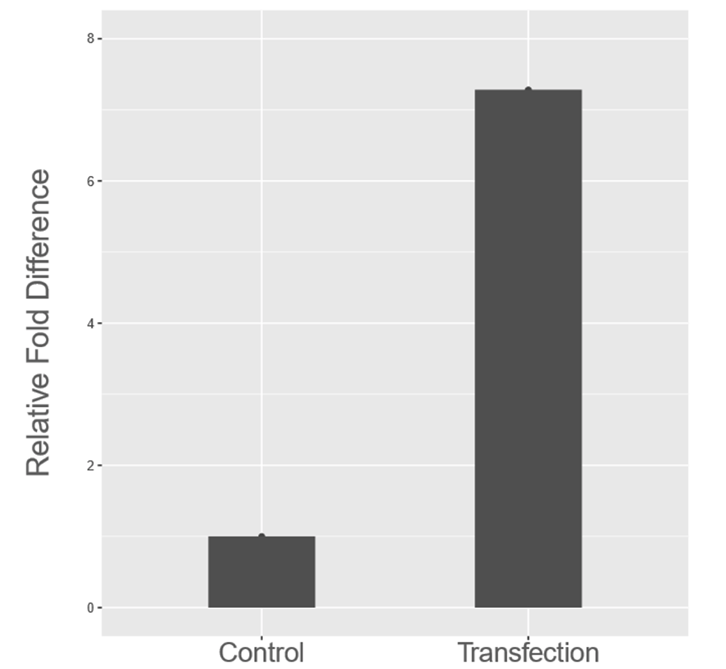
\includegraphics[width = 9cm]{fig3}
\centering
\vspace*{1\baselineskip}
\caption{{\bf Transfected MDA-MB-231 cell line exhibits PITPNC1 over-expression }
CRT-PCR confirmed a seven-fold amplification of PITPNC1 transcripts in the transduced MDA-MD-231 cell line.
}
\label{fig3}
\end{figure}
\vspace*{1\baselineskip}
\begin{figure}[H]
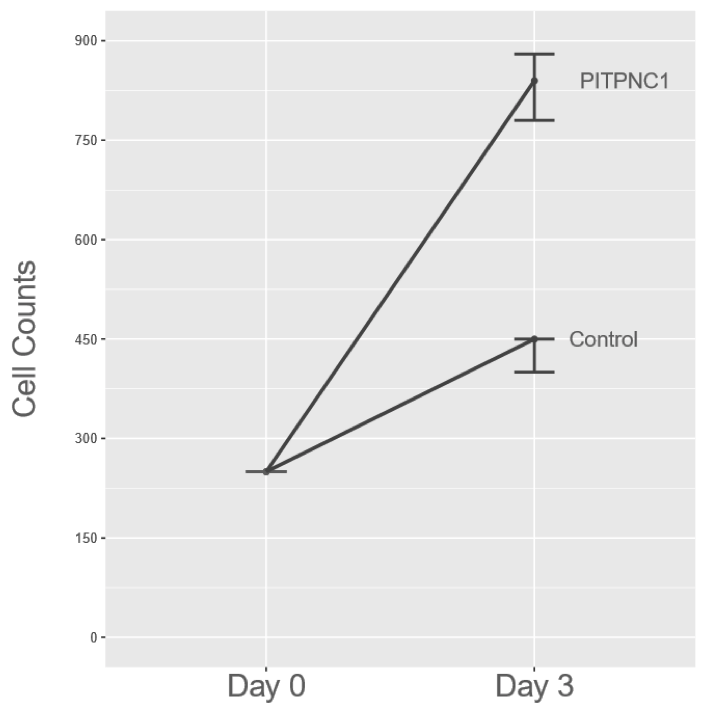
\includegraphics[width = 9cm]{fig4}
\centering
\vspace*{1\baselineskip}
\caption{{\bf PITPNC1 overexpression associated with increased proliferation}
250 cells from PITPNC1 transfected MDA-MB-231 cell line as well as transfection controls were plated and incubated for three days, after which cell numbers were counted using a hemocytometer. Bars represent summary statistics from technical replicates.
}
\label{fig4}
\end{figure}

\newpage
\section*{Discussion}
We showed that PITPNC1 is consistently amplified in both DCIS and IDC cases compared to normal breast samples, corroborating with the initial aCGH findings. Interestingly, PITPNC1 was amplified as early as DCIS and, as it is selected based on its association with poor prognosis and tumor grade, may be a candidate marker predictive of progression to invasion. Additionally, we have noticed an interesting trend of reduced PITPNC1 copy number associated with the DCIS to IDC transition. Although it is still unclear if PITPNC1 is functionally active in this process, it is certain that breast cancer progression may involve temporal down- and up-regulations at the genomic level, as seen in PITPNC1 copy number fluctuations cross successive tumor stage. The standard error for PITPNC1 fold difference is quite large, even with careful execution of experimental procedures on a fair large sample size. To control for unwanted confounding variables, additional quantification of PITPNC1 on matched DCIS and IDC with pure DCIS as control group would be necessary.

To test PITPNC1’S functional importance in the early development of breast cancer, we showed that PITPNC1 overexpression alone is enough to promote cell division and proliferation in a basal subtype cell line. As PITPNC1 protein is known to be involved in the transport of phosphatidylinositol, an important substrate upstream of EGF/PI3K pathway, it is plausible that PITPNC1 overexpression provide sufficient amount of precursor phosphatidylinositol to sustain PI3K/Akt function, leading to abnormal cell growth and proliferation. The EGFR/PI3K/Akt pathway has a prominent role in breast cancer progression, altered by mutations in a number of well-known genes, such as HER2, BRCA1, BRCA2, EGFR1, PIK3CA, PTEN, TP53, and RB. \cite{16_davis_sokolosky_stadelman_abrams_libra_candido_nicoletti_polesel_maestro_dassoro} The synergy between PITPNC1 and EGFR/PI3K/Akt pathway may indicate constitutive mutation or up-regulation of EGFR and of associated enzymes along the pathway; this is supported by elevated HER2 positive staining in the NKI dataset analysis. Therefore, amplification of PITPNC1 may be a requisite for the development of aggressive breast cancer and may promote fast entry into advanced invasive tumor stage. A comparison of proliferative potential of PITPNC1 overexpressed cell lines that do not over-express EGFR/HER2 will valid this hypothesis. Further biochemical assays, such as western blot and mass spectrometry, of proteins and metabolic intermediates abundance will confirm the importance of PITPNC1 in this pathway. As EGFR, while overexpressed, correlates with increased tumor grade and poorer prognosis, \cite{4_richard_sainsbury_needham_farndon_malcolm_harris_1987} mechanistic insights into PITPNC1 function may prove useful in anti-tumor drug development.

One thing to note is that we found no correlation between PITPNC1 overexpression and enhanced cell migration and invasion capabilities, which are landmarks for the DCIS to IDC transition. Many discrete processes are required for the development of invasive phenotype. Therefore, PITPNC1 amplification may not serve as a key genetic alteration crucial for invasion. As low quantity of cells was used to evaluate migration and invasion, it is necessary to reinforce this conclusion by performing qRT-PCR on genes involved in cell-to-cell adhesion and epithelial mesenchymal transition (EMT) in the transfected cell line.

Studies have established DCIS as a heterogeneous disease that can be categorized into distinct molecular subtypes. \cite{6_clark_warwick_carpenter_bowen_duffy_jones_2010} In additional to expression profiling, studies on tumor copy number aberrations have shown to aid in stratifying tumor cells into risk groups. \cite{19_wood_parsons_jones_lin_sjoblom_leary_shen_boca_barber_ptak,20_koboldt_fulton_mclellan_schmidt_kalicki-veizer_mcmichael_fulton_dooling_ding_mardis} Although some women can carry DCIS for their lifetime, many others develop invasive carcinomas, driven by their respective genomic landscape. Prognosis at this stage is intrinsically difficult; no convincing predictors of progression to invasive breast cancer has been identified. Although copy number aberrations in certain genes – c-MYC, HER2, FGFR1 - have been implicated in triggering invasive phenotype, \cite{14_cowell_weigelt_sakr_ng_hicks_king_reis-filho_2013} some proved otherwise. \cite{5_latta_tjan_parkes_omalley_2002} Additionally, identifying the exact timing of disease associated copy number aberrations during the course of cancer progression may prove both challenging and crucial toward understanding its role in pathogenesis. \cite{7_corzo_corominas_tusquets_salido_bellet_fabregat_serrano_sol_2006,8_robanus-maandag_bosch_kristel_hart_faneyte_nederlof_peterse_van} Here we showed that amplification of PITPNC1 occurs early in breast cancer progression and promote cell proliferation, possibly in the EFR/PI3K pathway. PITPNC1 is important in early development of breast cancer but may not directly enhance tumor invasion.

Identification of driver mutations at a single gene level and determination of their respective contribution to the enhanced invasive potential of cancer cells, via expression profiling and functional assays, are indispensable steps toward elucidating breast cancer pathobiology. These critical molecular events underlying breast cancer transition and progression have profound implications for early breast cancer diagnosis and therapeutics.

\medskip
\printbibliography

\end{document}
